\documentclass[a4paper]{article}

\usepackage{amsfonts, amsmath, amssymb, amsthm}
\usepackage{fullpage}
\usepackage{float}
\usepackage{graphicx}
\usepackage[bottom,flushmargin]{footmisc}

\setlength{\parindent}{0pt}

\renewcommand{\O}{\mathcal{O}}
\newcommand{\Z}{\mathbb{Z}}
\newcommand{\R}{\mathbb{R}}

\newtheorem*{theorem}{Theorem}
\newtheorem*{corollary}{Corollary}

\begin{document}
	\title{How To \textit{Lights Out}}
	\author{William Boyles}
	\date{\today}
	\maketitle
	
	\section{How Do I Play?}
	\textit{Lights Out} is a handheld game manufactured by Tiger Electronics and released in 1995.
	The game board consists of a $5 \times 5$ grid of lights which are also buttons.
	The player is presented with a seemingly random pattern of lights that are either on or off.
	Whenever the player clicks any light in the grid, the on/off status of that light and any lights above, below, left or right of it are toggled.
	The player wins the game when they find a series of light presses that result in all lights being in the off state, ideally in as few clicks as possible.
	
	\begin{figure}[H]
		\centering
		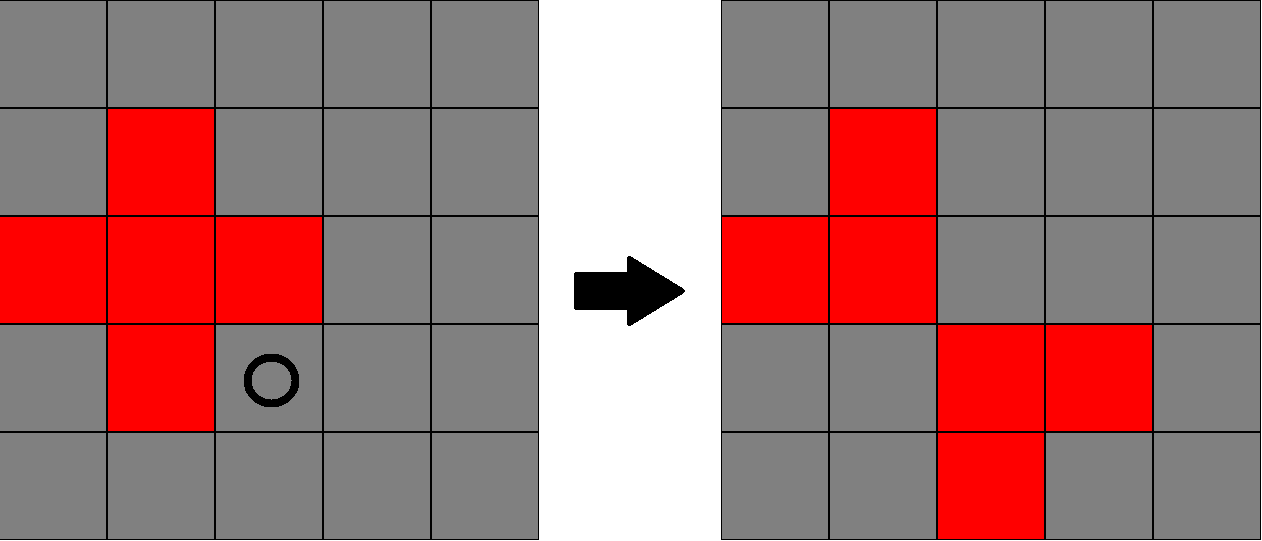
\includegraphics[width=\textwidth]{board0.png}
		\caption{Clicking the circled light toggles its state and the state of its neighbors}
	\end{figure}

	\section{How Do I Win?}
	\subsection{Reduce the Number of On Lights (A Bad Strategy)}
	One of the first strategies that someone might try to solve a \textit{Lights Out} board is to only make moves that decrease the number of lights in the on state.
	However, using the number of on lights as a metric for progress towards solving a board is not a very useful metric.
	For example, the board on the left has 20 on lights and can be solved in at least 6 clicks, while the board on the right has 1 light on and can be solved in at least 11 clicks.
	
	\begin{figure}[H]
		\centering
		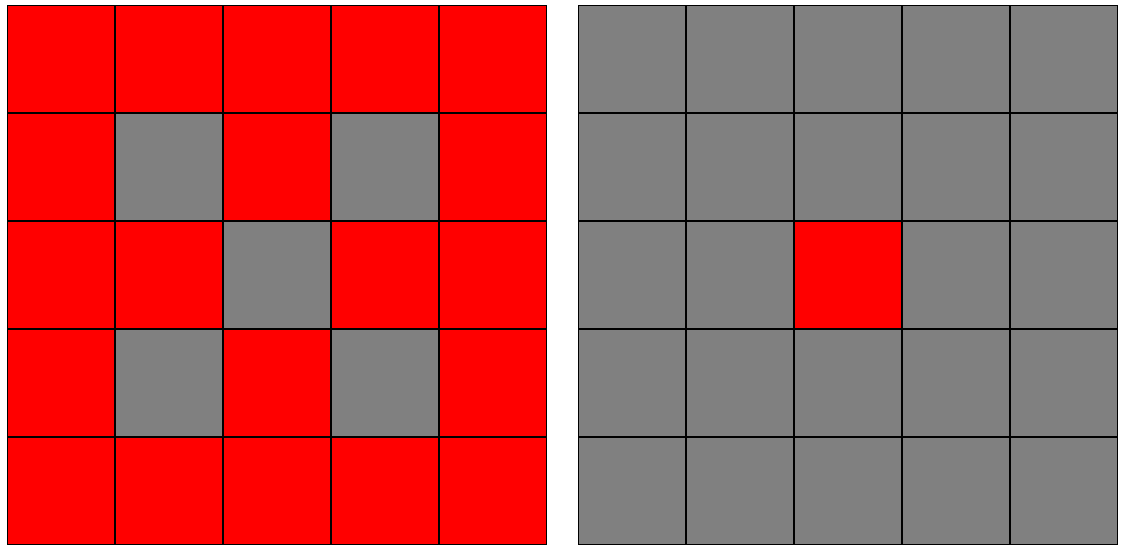
\includegraphics[width=\textwidth]{board1.png}
		\caption{Fewer on lights does not mean closer to being solved}
	\end{figure}

	Further, for the board on the right, there are no moves that decrease or even keep the number of lights the same.
	So, the strategy fails in this case.
	
	\subsection{Light Chasing (Making a 2D Problem 1D)}
	We want a rule that will 
	\begin{enumerate}
		\item
			Reduce the ``complexity'' of the board
		\item
			Will never tell us there aren't any buttons to click while the board is not solved
	\end{enumerate}
	Here's one idea that certainly satisfies the first condition: Whenever a light is on, we'll click the light immediately below it.
	This will turn off the on light.
	If we do this for every light in a row, then an entire row of lights will be off.
	If we do this working from the top of the board to the bottom, we can turn off every light in every row except the last one.
	
	\begin{figure}[H]
		\centering
		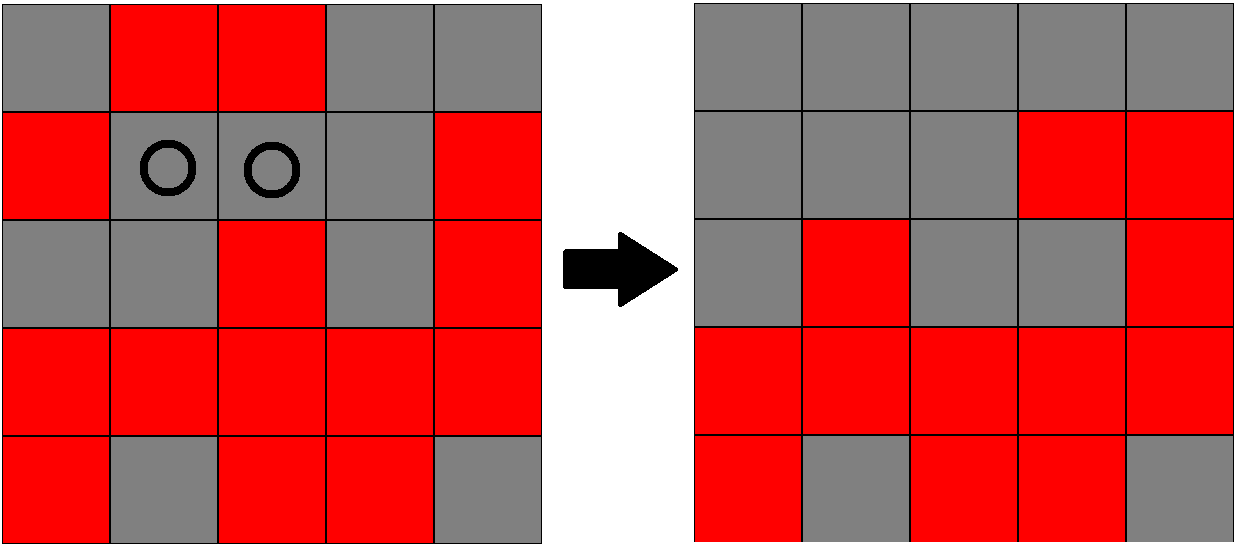
\includegraphics[width=\textwidth]{board2.png}
		\caption{Light chasing clears rows}
	\end{figure}

	After executing the light chasing strategy on many scrambled boards, you may notice that there are only a small number of patterns that appear in the bottom row.
	\begin{figure}[H]
		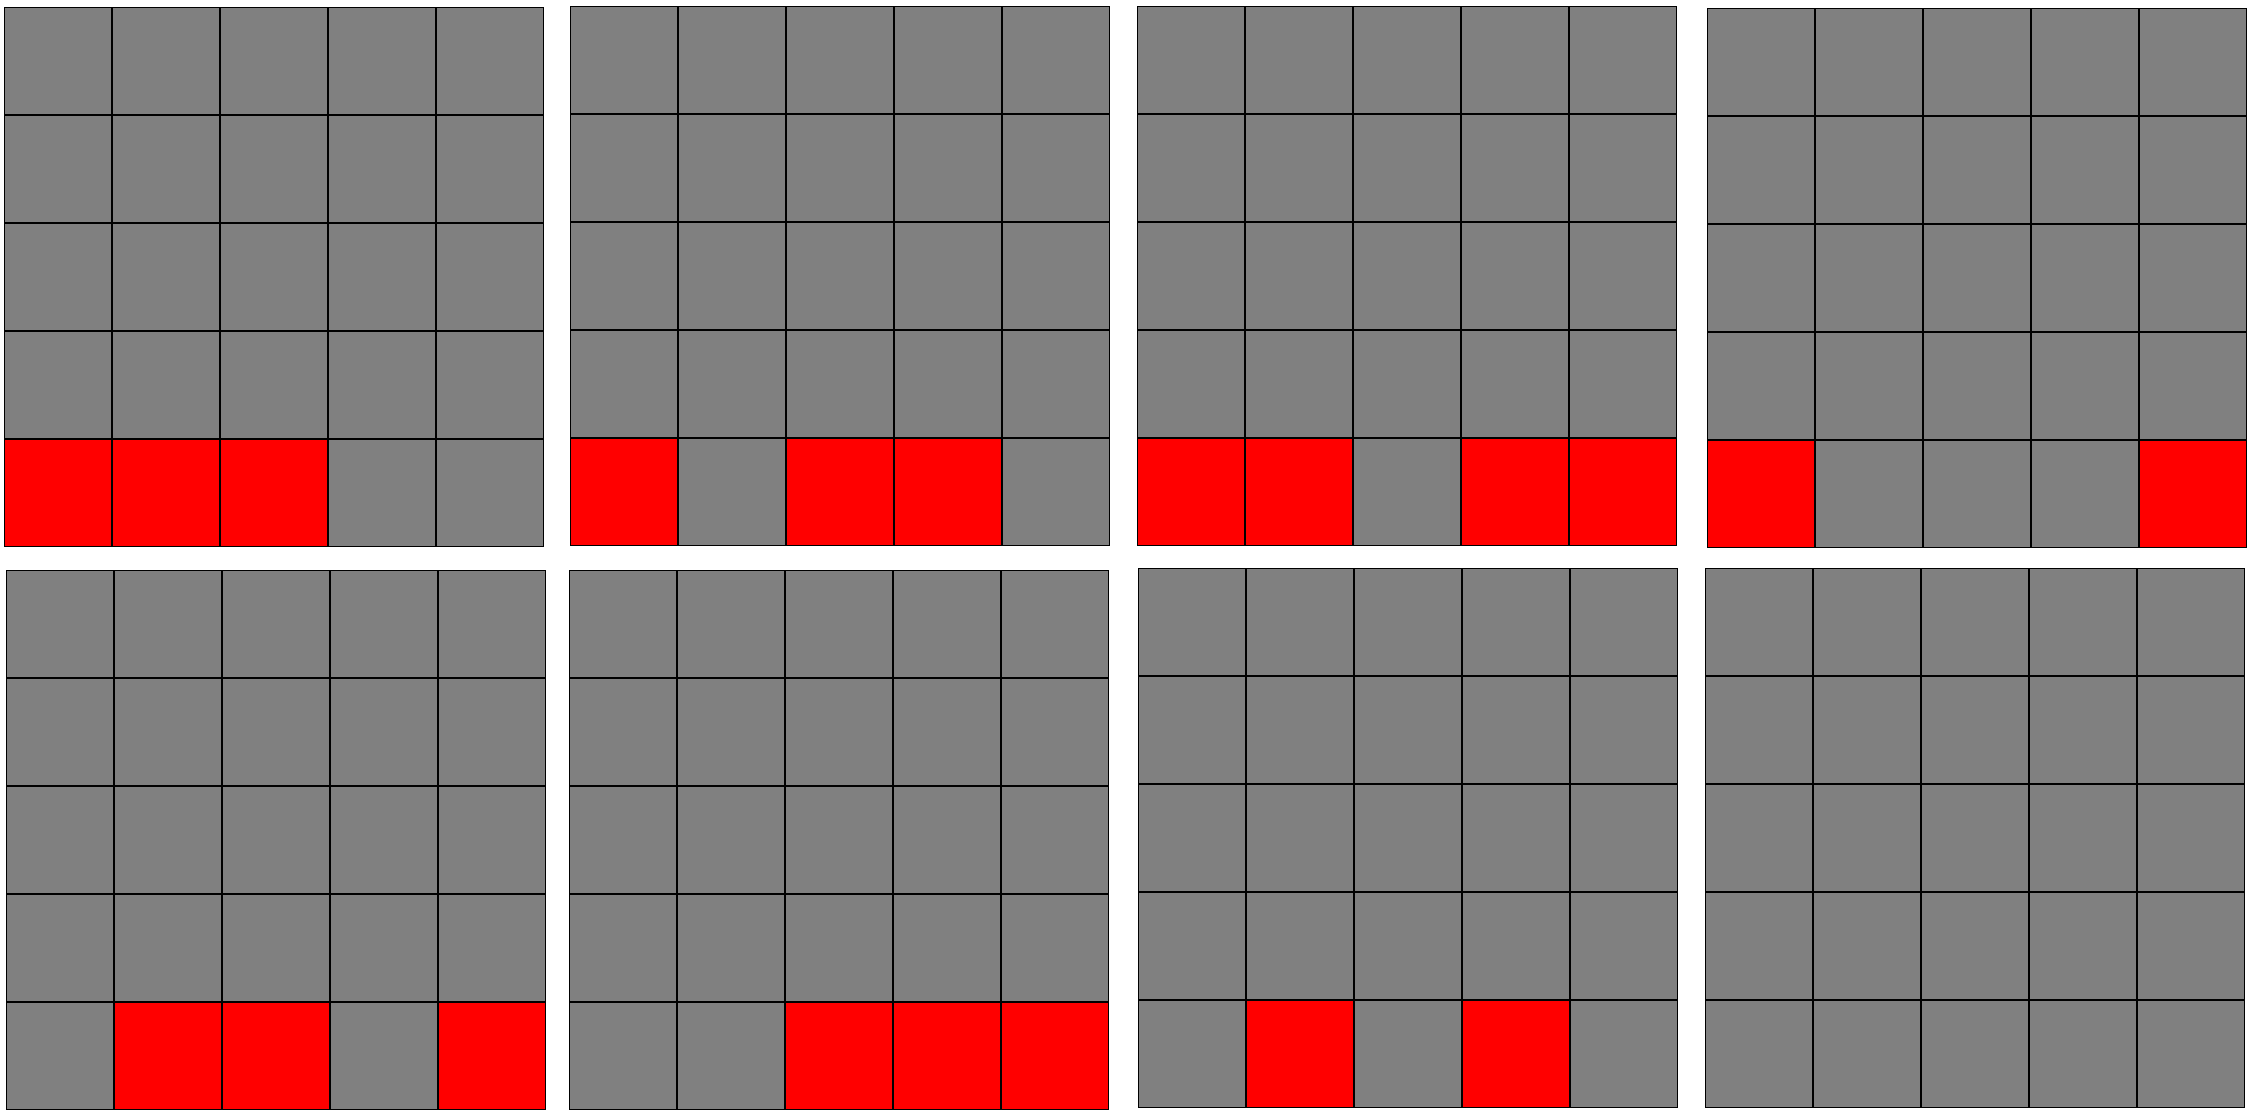
\includegraphics[width=\textwidth]{board3.png}
		\caption{A $5 \times 5$ board has 8 bottom row patterns after light chasing. One is a solved board.}
	\end{figure}
	If we can find a series of light presses that ``cancel out'' these last row patterns, then we would have solved the board. \\
	
	Since our strategy already uses light chasing, one idea to handle the last row is to make some moves elsewhere on the board and then perform lightchasing again to clear the bottom row.
	We can notice that any moves we do in any row except the top row will have no effect after light chasing, as our initial move will turn on a light in an above row, meaning we will click in the same spot as our initial move\footnote{We can prove that the same set of clicks in any order have the same net effect, and clicking a light twice is the same as not clicking it at all.}.
	So, we only need to consider moves in the top row.
	We can click each button in the top row and light chase it down to see its effect on the bottom row.
	
	\begin{figure}[H]
		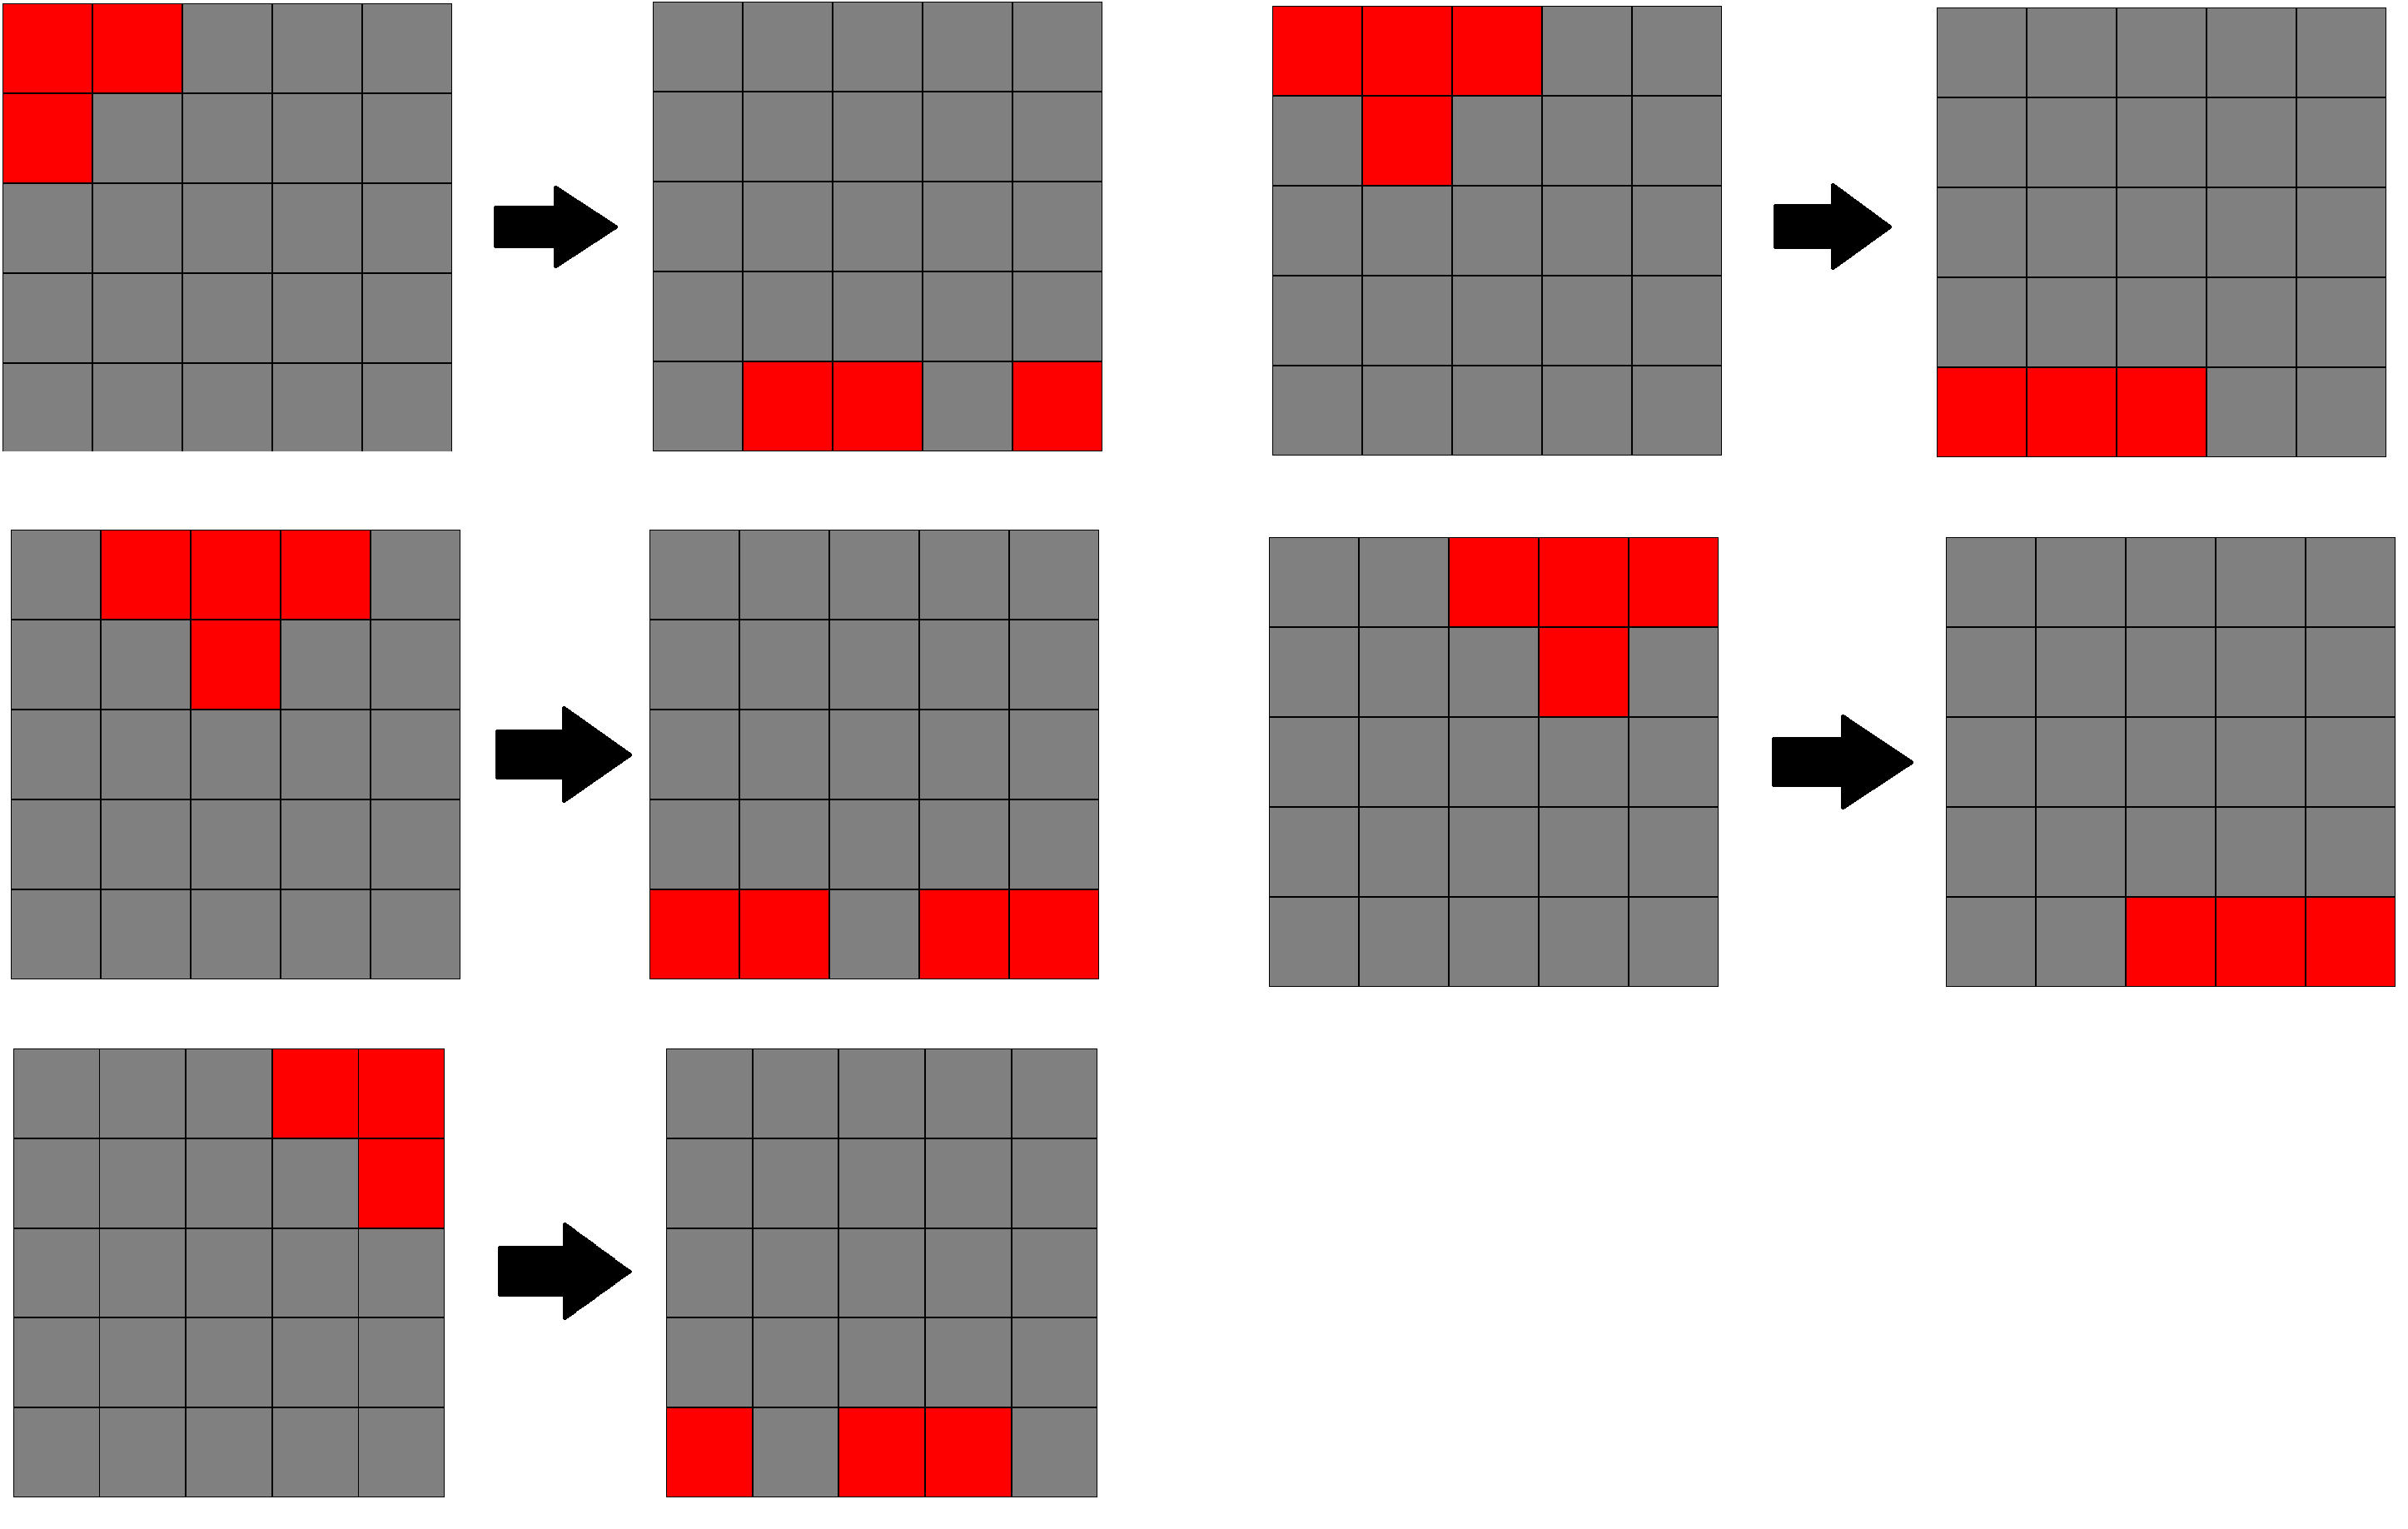
\includegraphics[width=\textwidth]{board4.png}
		\caption{Effect of light chasing after clicking each light in the top row}
	\end{figure}

	We can immediately see solutions to most of our bottom row patterns.
	For the remaining ones, we can notice that the desired bottom row patterns are the sum, modulo 2, of the results of single-button light presses.
	Since the result of applying two sequences of light presses is just the sum, modulo 2, of their individual parts\footnote{We'll more rigorously justify this fact later.}, we now have a full strategy for solving a given \textit{Lights Out} board.
	Further, our general approach of light chasing, finding a top row strategy, and light chasing again generalizes to boards of different sizes.
	
	\section{How Do I Win Optimally?}
	After executing the full solving strategy a few times, we can notice that our strategy does not give solutions that use as few clicks as possible, even for boards that can be solved in a small number of clicks.
	
	\subsection{Don't Push Buttons Twice}
	For example, consider a board generated by clicking a single light in the top row.
	We can certainly solve this board in one move by clicking the same light in the top row.
	However, our strategy would have us chase the lights to the bottom row, at which point we'd realize which light we need to click in the top row, and we'd still need to chase the lights down again.
	
	\begin{figure}[H]
		\centering
		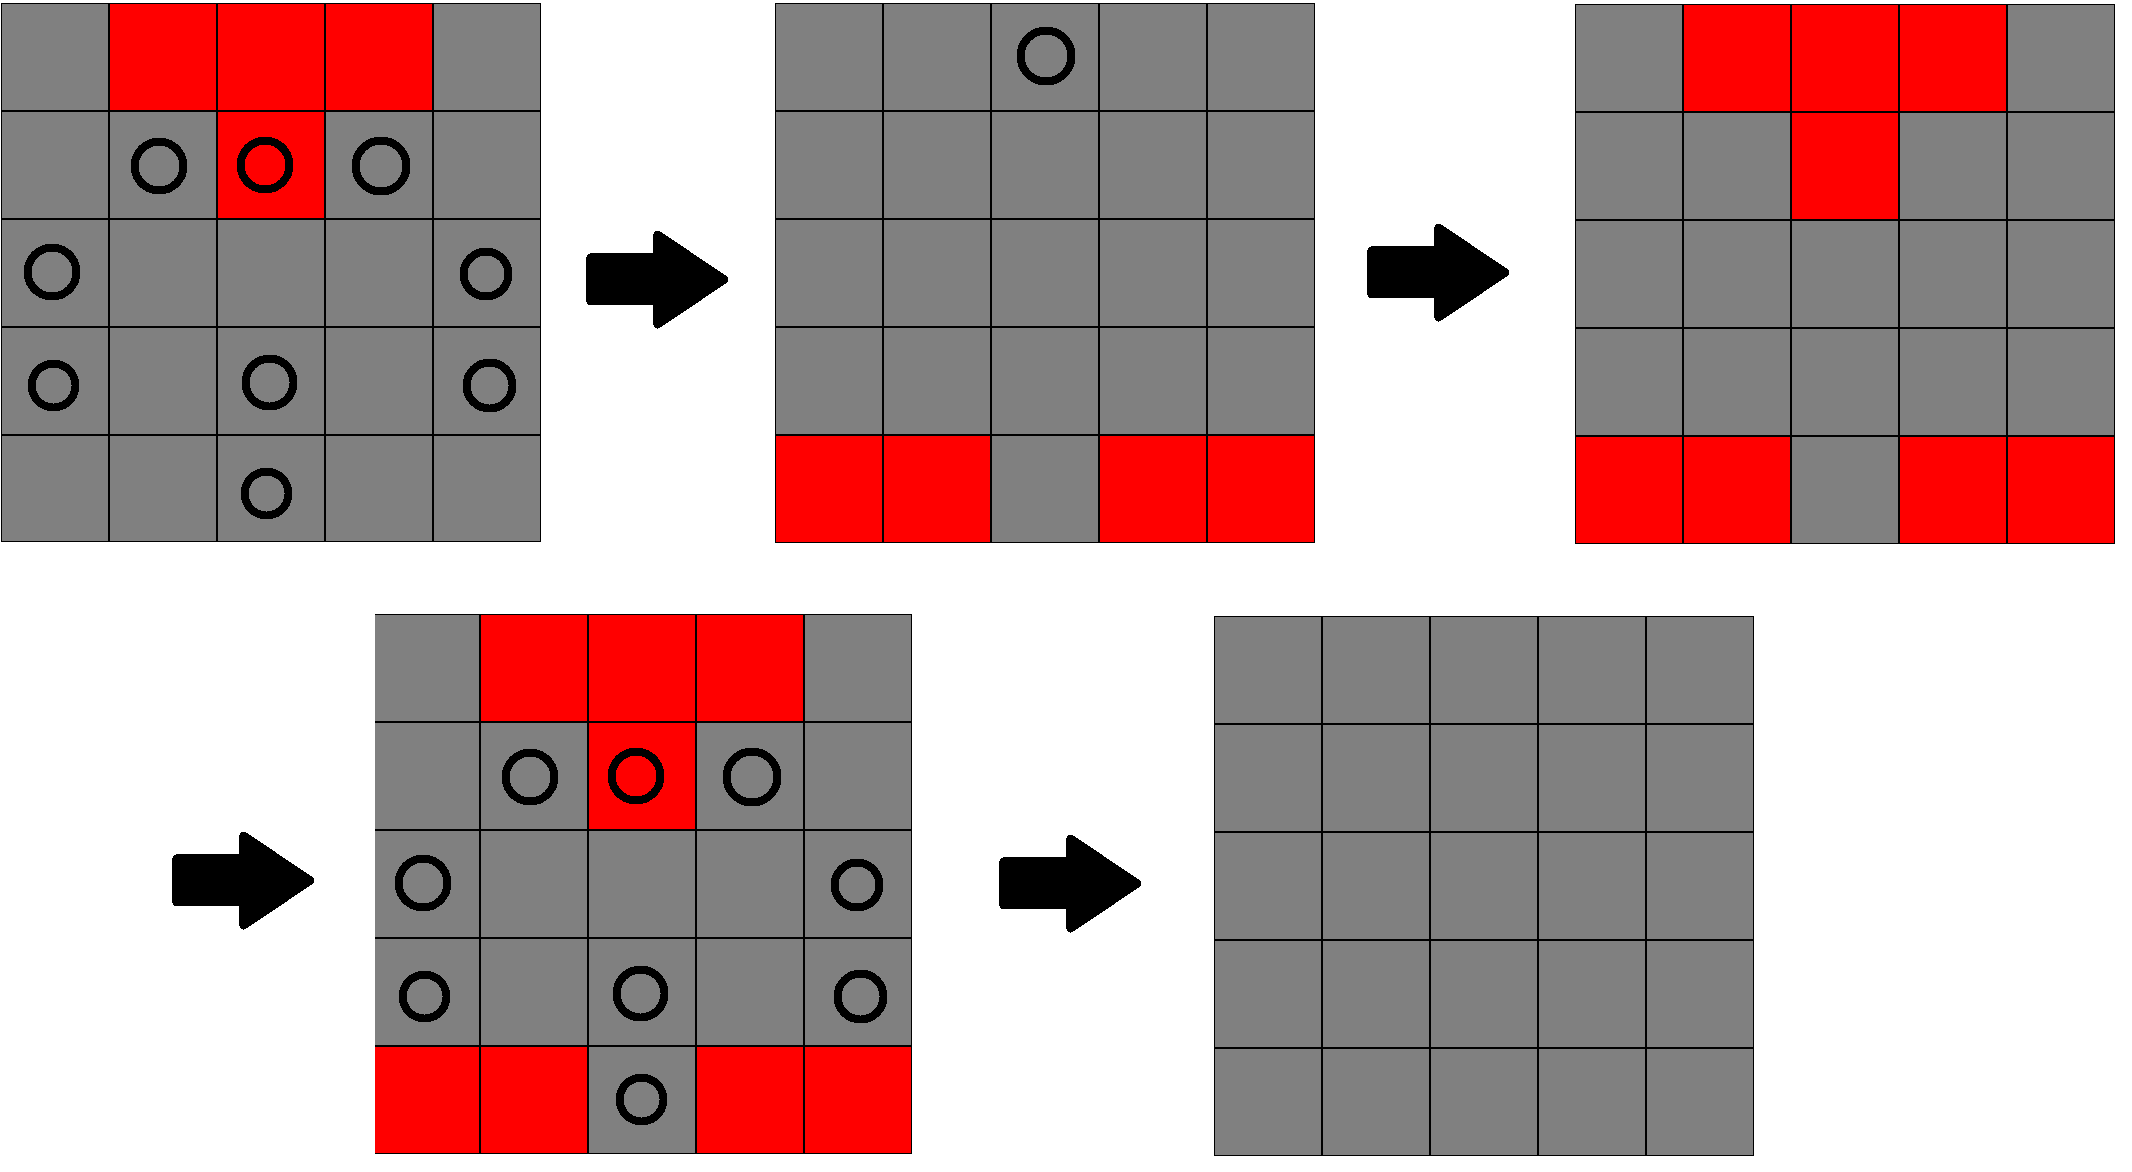
\includegraphics[width=\textwidth]{board5.png}
		\caption{Light chasing strategy can give highly non-optimal solutions}
	\end{figure}

	We can see from this example that we're pushing many of the same buttons twice.
	Since pushing a button twice is the same as not pushing it at all, this is where the redundancy comes from.
	
	\subsection{Remove Quiet Patterns}
	Even after eliminating redundant clicks of the same button from a solution, it may still not be optimal.
	Consider the board created by clicking the 1st, 3rd, and 5th lights in the top row of a $5 \times 5$ board.
	The solution found by light chasing with duplicate clicks removed has 9 clicks.
	However, this board can also be solved in 3 clicks the same way it was created.
	
	\begin{figure}[H]
		\centering
		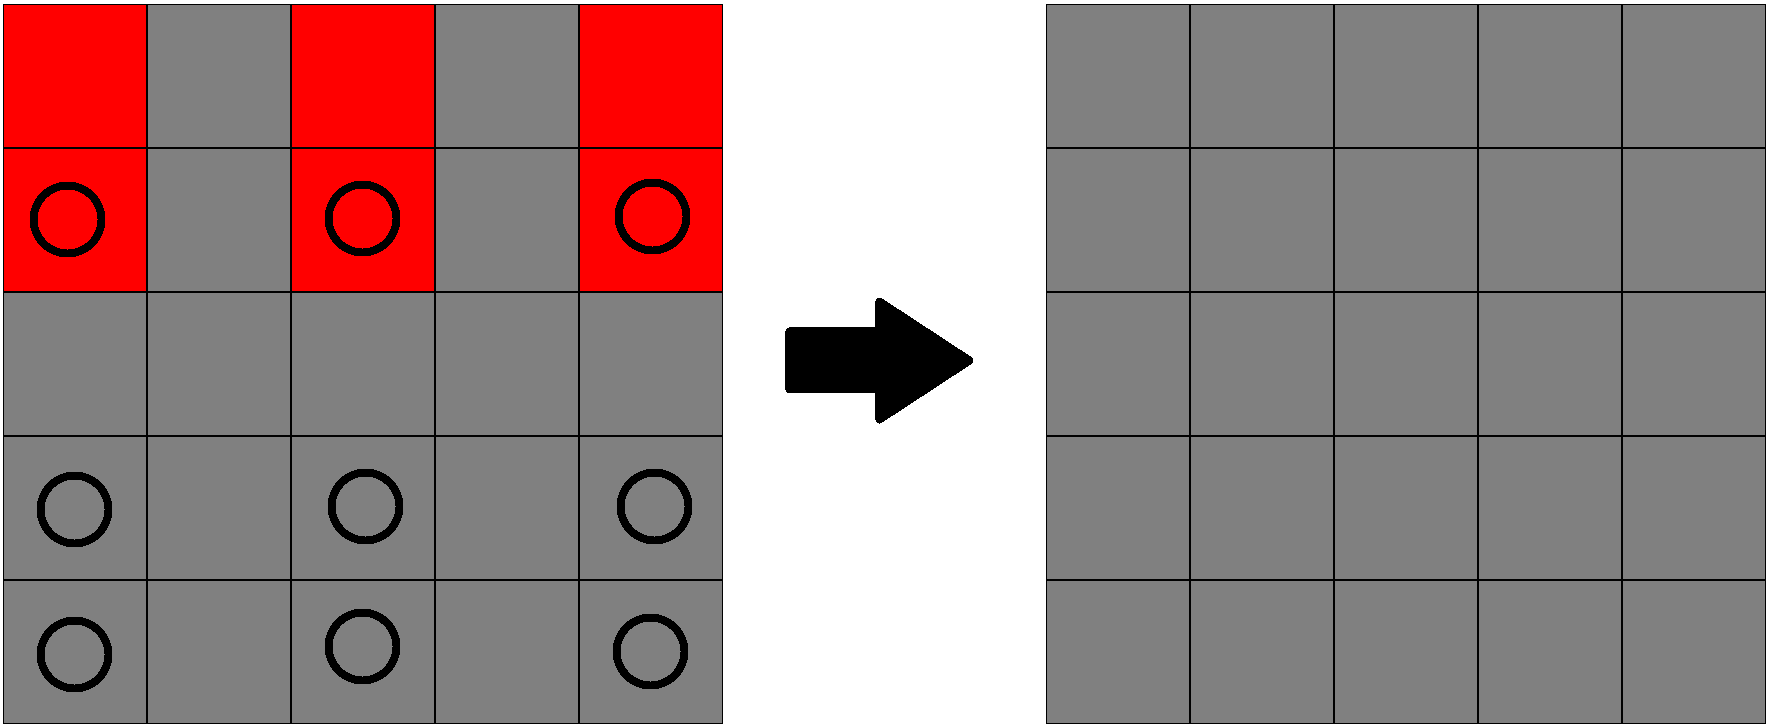
\includegraphics[width=\textwidth]{board6.png}
		\caption{Even after removing redundant clicks, light chasing may not give optimal solutions}
	\end{figure}

	Let's consider what's happening here mathematically.
	We can represent the state of our board as a $5 \times 5$ matrix with entries that are either 0 or 1.
	Let $T$ be the linear\footnote{We'll justify that it's linear later} function that takes a $5 \times 5$ matrix of 0 and 1 entries representing button presses and returns the $5 \times 5$ matrix representing the state of a board after pressing those buttons.
	Let $S$ represent our starting board to which we're trying to find a solution.
	Let $A_3$ represent the solution of clicking the 3 buttons in the top row.
	Let $A_9$ represent the solution obtained from light chasing that uses 9 clicks.
	Let $\mathbf{0}$ be the $5 \times 5$ 0 matrix.
	Then working modulo 2,
	\begin{align*}
		S + T(A_3) &= \mathbf{0} = S + T(A_9) \\
		T(A_3) &= T(A_9) \\
		T(A_3) + T(A_9) &= \mathbf{0} \\
		T(A_3 + A_9) &= \mathbf{0} = T(\mathbf{0})
	\end{align*}
	However, we can see that $A_3 + A_9 \neq \mathbf{0}$.
	So, $A_3 + A_9$ is a sequence of button presses that have no net effect on the board.
	Therefore, if $B$ is a sequence of light presses, then
	\begin{equation*}
		T(B) = \mathbf{0} + T(B) = T(A_3 + A_9) + T(B) = T(A_3 + A_9 + B).
	\end{equation*}
	So $A_3 + A_9 + B$ is an equivalent solution.
	We call any series of button presses with this no net effect property a ``quiet pattern'' or ``null pattern'' because it's in the null space of $T$. \\
	
	Equivalent solutions like $A_3$ and $A_9$ always differ by a quiet pattern.
	So, to find an optimal solution, we need to find any solution, and apply every quiet pattern to see if any equivalent solutions use fewer clicks. 
	
	\subsection{How Do I Find Quiet Patterns?}
	\subsubsection{The Linear Algebra Way}
	We are looking for every element in $\ker T$.
	So, it would be a good idea to write $T$ in a form we know how to systematically find the kernel of, namely a matrix.
	In \cite{anderson_feil}, Anderson and Fiel showed that $T$ is a $n^2 \times n^2$ matrix with the following block form
	\begin{equation*}
		T = \begin{bmatrix}
			B & I & O & O & O & \dots & O \\
			I & B & I & O & O & \dots & O \\
			O & I & B & I & O & \dots & O \\
			\vdots & \ddots & \ddots & \ddots & \ddots & \ddots & \vdots \\
			O & \dots & O & I & B & I & O \\
			O & \dots & O & O & I & B & I \\
			O & \dots & O & O & O & I & B
		\end{bmatrix}
	\end{equation*}
	where $I$ is the $n \times n$ identity matrix, $O$ is the $n \times n$ zero matrix, and
	\begin{equation*}
		B = \begin{bmatrix}
			1 & 1 & 0 & 0 & 0 & \dots & 0 \\
			1 & 1 & 1 & 0 & 0 & \dots & 0 \\
			0 & 1 & 1 & 1 & 0 & \dots & 0 \\
			\vdots & \ddots & \ddots & \ddots & \ddots & \ddots & \vdots \\
			0 & \dots & 0 & 1 & 1 & 1 & 0 \\
			0 & \dots & 0 & 0 & 1 & 1 & 1 \\
			0 & \dots & 0 & 0 & 0 & 1 & 1
		\end{bmatrix}.
	\end{equation*}
	Row reducing $T$, we can find the dimension of $\ker T$.
	Looking at the last $\lvert \ker T \rvert$ columns of $T$ after row reduction, we have the basis vectors for $\ker T$, which are exactly the quiet patterns. \\
	
	Since the matrix is of $n^2 \times n^2$ size, applying the standard row reduction algorithm will take $\O(n^6)$ time, where $n$ is the sidelength of the board.
	
	\subsubsection{The Light Chasing Way}
	As Anderson and Feil allude to in \cite{anderson_feil}, we can more quickly find quiet patterns by taking advantage of light chasing.
	When we were developing our light chasing strategy to solve a given board, we were looking for combinations of button presses in the top row that would cancel out the on lights in the bottom row.
	We can use the same approach to find quiet patterns by looking for combinations of button presses that have no effect on the bottom row.
	For example, for the $5 \times 5$ board, we're looking for a row vector $\vec{t}$ such that
	\begin{equation*}
		\vec{t}\begin{bmatrix}
			0 & 1 & 1 & 0 & 1 \\
			1 & 1 & 1 & 0 & 0 \\
			1 & 1 & 0 & 1 & 1 \\
			0 & 0 & 1 & 1 & 1 \\
			1 & 0 & 1 & 1 & 0
		\end{bmatrix} = \vec{0},
	\end{equation*}
	where $\vec{0}$ is the row vector with five 0 elements.
	$\vec{t} = \begin{bmatrix} 1 & 0 & 1 & 0 & 1 \end{bmatrix}$ is one such solution.
	For a $5 \times 5$ board, there are 4 quiet patterns, once of which is trivially $\vec{t} = \vec{0}$. \\
	
	We're  guaranteed that each quiet pattern we find will be unique because it will differ from any other quiet pattern we find in the first row.
	We're also guaranteed that this approach will find all quiet patterns.
	Any clicks in the bottom $n-1$ rows would create on lights in the above row, which would need to be canceled by a light press in one of the two rows above. \\
	
	Calculating the results of the bottom row requires $\O(n^2)$ clicks to light chase.
	Since we need to do this once per each light in the top row, it takes $\O(n^3)$ time to calculate this $n \times n$ matrix.
	Then any row reducing to find a basis for the kernel of this matrix also takes $\O(n^3)$ time.
	So, the overall running time is $\O(n^3)$, much better than the linear algebra approach.
	
	\subsection{How Hard Is Optimizing a Solution?}
	In the worst case, $\dim{(\ker{T})} \in \O(n)$, where $n$ is the number of buttons on the board.
	So, to enumerate every vector in $\ker{T}$ requires $\O(2^n)$ time.
	Therefore, finding an optimal solution to boards where $\dim{(\ker{T})}$ is large is likely not computationally quick.
	In \cite{CHEN200493}, Chen, Li, Zhang, and Wang consider only solutions to the board pattern with all lights on.
	They find that even for this single solution, the problem of finding a minimal solution is NP-Complete for general graphs.
	However, they find that for certain classes of simple graphs, like trees, unicyclic, and bicyclic, that one can find an optimal solution in $\O(n)$ time, where $n$ is the number of vertices in the graph.
	
	\section{When Is a Board Solvable?}
	We can easily extend our solving strategy to get light patterns we want by thinking of a light as ``on'' when it's not in the desired state.
	However, there are some light patterns that are impossible to get starting from a blank board.
	For example, we cannot have a board state where only a single light in any corner is on.
	So, how do we know by looking at a pattern of lights if it's solvable? \\
	
	Anderson and Feil in \cite{anderson_feil} gave an answer in terms of quiet patterns.
	\begin{theorem}[Anderson and Feil]
		A light pattern $\vec{b}$, represented as a column vector, is solvable if and only if it is perpendicular to all quiet patterns.
	\end{theorem}
	Since we're working with elements in the finite field $\Z_2$, perpendicular is a bit of a strange idea, since a vector is perpendicular to itself.
	If we want to think of the vectors and coming from a field like $\Z$ or $\R$, we can redefined the notion of perpendicular to mean that the dot product is even.
	\begin{corollary}
		For any board size where $\dim{(\ker{T})} = 0$, all light patterns are achievable.
	\end{corollary}
	\begin{corollary}
		Only 1 our of every $2^{\dim{(\ker{T})}}$ boards are solvable.
	\end{corollary}

	\subsection{Are Certain Patterns Always Solvable?}
	In \cite{Sutner1989}, Sutner proved the following:
	\begin{theorem}[Sutner]
		For any board represented as an undirected graph\footnote{An  $n \times n$ board is a grid graph}, the board state with all lights on is always solvable.
	\end{theorem}
	This gives us some neat results about which boards are solvable.
	
	\begin{corollary}
		Let $\vec{b}$ be a light pattern.
		Define $-\vec{b}$ to be the light pattern with all light states inverted.
		$\vec{b}$ is solvable if and only if $-\vec{b}$ is solvable.
	\end{corollary}
	\begin{corollary}
		Let $\vec{n} \in \ker{T}$.
		Then the light pattern represented by $\vec{n}$ is solvable.
	\end{corollary}
	\begin{corollary}
		All elements in $\ker{T}$ contain an even number of 1's.
	\end{corollary}

	Now that we know the ``inverse'' of a board pattern is also solvable, we can almost think of the collection of solvable boards under the operation of light presses as an Abelian group\footnote{Not quite a group because as we alluded to, inverses are not unique.}.

	\section{Can We Find $\dim{(\ker{T})}$ Quickly?}
	Although we've already seen that it's unlikely that there is a fast way to find minimal solutions to board states when $\dim{(\ker T)} \in \O(n)$, perhaps we can find when the dimension is smaller and focus on these examples. \\
	
	In \cite{HUNZIKER2004465}, Hunziker, Machiavelo, and Park show the following.
	\begin{theorem}[Hunziker, Machiavelo, and Park]
		Let $F_n(x) = U_{n-1}(x/2)$ where $U_{n-1}(x)$ is the Chebyshev polynomial of the second kind of degree $n-1$.
		Let $f_n(x) = F_n(x) \mod 2$.
		Then $\dim{(\ker T)}$ is the degree of the polynomial $\gcd{(f_{n+1}(x),f_{n+1}(1-x))}$.
	\end{theorem}
	This derives from taking the matrix representation of $T$ with $x$'s along the main diagonal instead of 1's.
	
	\section{Are There Extensions of \textit{Lights Out}?}
	\subsection{Graphs}
	The most common way to characterize problems related to \textit{Lights Out} that extend to the structures on would be interested is simple graphs.
	In this case, we define a graph $G = (V,E)$ where lights are represented by vertices and their connections to other lights represented by edges.
	So, pushing a light $v \in V$ toggles all lights in the set $N(v) = \{u \in V \mid uv \in E\} \cup \{v\}$.
	For the $n \times n$ board we've been focused on, it would be an $n \times n$ grid graph.
	
	\subsubsection{Parity Covers}
	Now with a graph-theoretical perspective, we can restate the problem of looking for a solution to all lights being on.
	We are looking for some $V^* \subseteq V$ such that for all $v \in V$, $\lvert N(v) \cap V^* \rvert$ is odd.
	This is called an odd parity cover.
	If we instead require that $\lvert N(v) \cap V^* \rvert$ is even, we have an even parity cover, which corresponds to a quiet pattern.
	We even restate the general problem of solving some light pattern.
	Given some starting set of on lights $S \subseteq V$, we are looking for $V^* \subseteq V$ such that for all $v \in V$, $\lvert N(v) \cap V^* \rvert$ is odd if $v \in S$ and even otherwise.
	
	\subsection{$\sigma$ Rule}
	The rule that a light toggles itself and its neighbors is called a $\sigma^+$ rule.
	If we instead remove $v$ from $N(v)$ so that pressing a light does not toggle itself, we have a $\sigma$ rule.
	Interestingly, on the same graph, ``eigenboards'' (i.e. $T\vec{t} = \vec{t}$) with a $\sigma^+$ rule are exactly the quiet patterns with a $\sigma$ rule.
	Likewise, eigenboards with a $\sigma$ rule are exactly the quiet patterns with a $\sigma^+$ rule.
	At least for $n \times n$ grid graphs, eigenboards behave very nicely and are easy to find and fully characterize, which seems to imply that finding optimal solutions to $\sigma$ \textit{Lights Out} boards is much easier than for $\sigma^+$.
	
	\subsection{Many States}
	We've focused on buttons that only have two states $\{0,1\}$ representing on and off.
	However, we could also think about buttons have a set of states $\{0,1,\dots,k-1\}$ representing $k$ distinct states, where pushing a light $v$ increments the state of every light in $v$'s neighborhood modulo $k$.
	
	\subsection{On Lights Only}
	In the original problem, the player is allowed to push any light at any time, regardless of its state.
	However, we could restrict the player to only pushing lights that are currently in the ``on'' state.
	Suprisingly, Goldwasser, Wang, and Wu show in \cite{GOLDWASSER2009774} that any board that is solvable under a $\sigma^+$ rule with no restriction on button presses is also solvable with the lit-only restriction.

	\newpage
	\bibliography{refs.bib}
	\bibliographystyle{amsplain}
\end{document}